\documentclass[border = 3mm]{standalone}
\usepackage{tikz}

\begin{document}
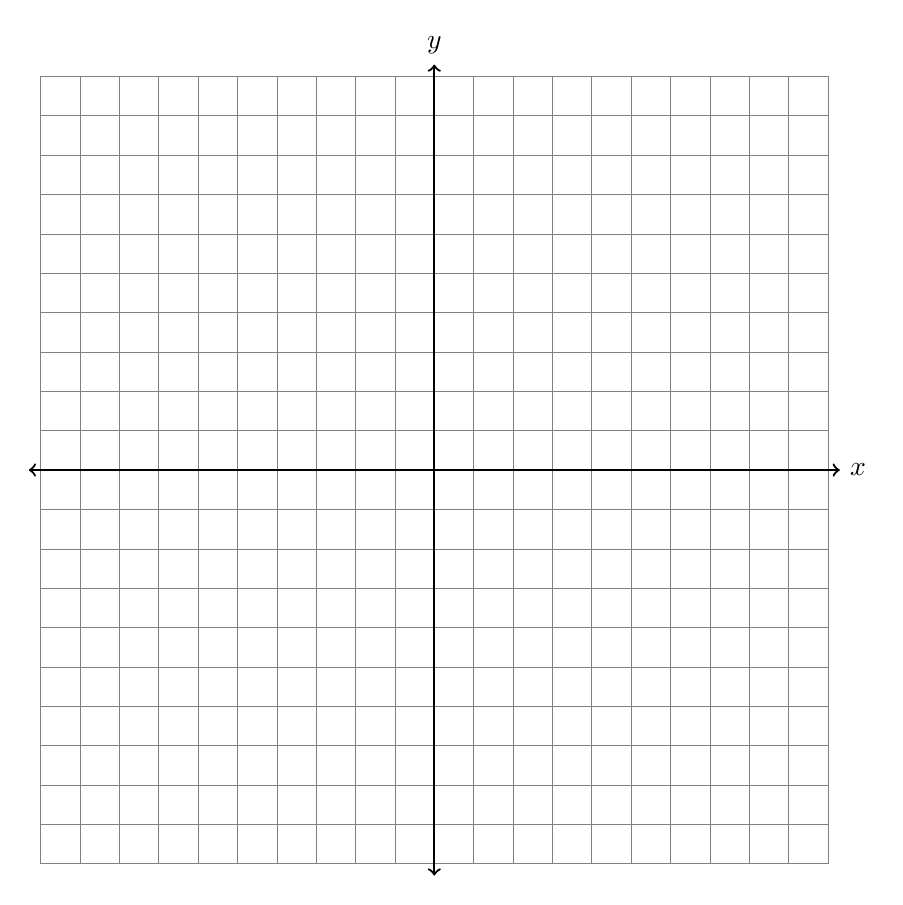
\begin{tikzpicture}


  % grid black help lines default colour is black!40
  \draw[help lines, step = 0.5cm] (-5, -5) grid (5, 5);

  % axis with end labels
  \draw[thick, <->] (0, -5.15) -- (0, 5.15) node[above] {$y$};
  \draw[thick, <->] (-5.15, 0) -- (5.15, 0) node[right] {$x$};

\end{tikzpicture}
\end{document}